\documentclass{standalone}
\usepackage{tikz}

\begin{document}

\centering

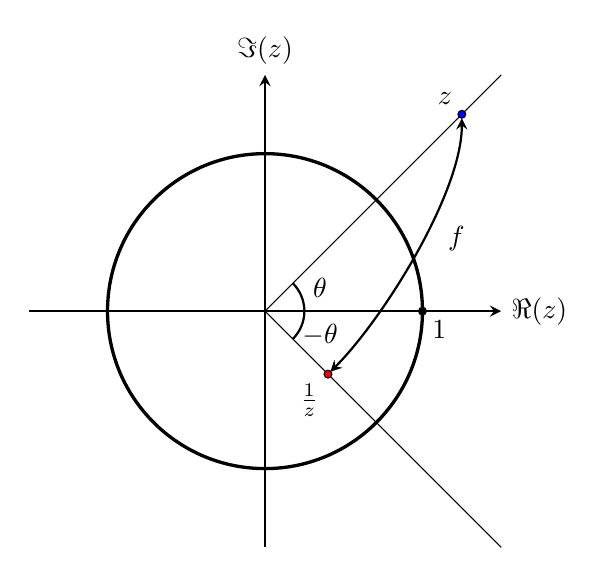
\begin{tikzpicture}[>=stealth]
    \tikzset{
    every node/.style={font=\normalsize, text=black},
    arrowstyle/.style={->, >=stealth}}
    %Assen
    \draw [thick, arrowstyle](0,-3) -- (0,3) node[above]{$\Im(z)$};
    \draw [thick, arrowstyle](-3,0) -- (3,0) node[right]{$\Re(z)$};
    
    %Eenheidscirkel
    \draw[very thick] (0,0) circle(2);
    \draw[fill=black] (2,0) circle (0.05);
    \node[below right] at (2,0) {1};
    
    %coordinaten
    \coordinate (z2) at (2.5,2.5);
    \coordinate (z4) at (0.8,-0.8);

    \draw [-](0,0) -- (3,3);
    \draw [-](0,0) -- (3,-3);
    %z
    \draw[fill=blue] (z2) circle(0.05) node[above left] {$z$};
    %Reciproque
    \draw[fill=red] (z4) circle(0.05) node[below left] {$\frac{1}{z}$};
    
    % Cirkelboogje tekenen voor de hoek theta
    \draw[thick] (0.5,0) arc[start angle=0, end angle=45, radius=0.5];
    \draw[thick] (0.5,0) arc[start angle=0, end angle=-45, radius=0.5];

    % Label voor theta
    \node at (0.7,0.3) {$\theta$};
    \node at (0.7,-0.3) {$-\theta$};
    \draw[stealth-stealth, thick]
    [black] (2.5,2.45)
    .. controls (2.5,1.5) and (1.5,-0.1) .. (0.83,-0.77);
    \node[below right,black] at (2.2,1.2) {$f$};

\end{tikzpicture}

\end{document}